%\documentclass[preprint, review, 3p, authoryear]{elsarticle}
\documentclass[10pt, a4paper]{article}

\usepackage{setspace}
\usepackage[utf8]{inputenc}
\usepackage{marginnote}
\usepackage{amsmath, amssymb, amsthm}
\usepackage{xcolor}
\usepackage{graphicx}
\usepackage[authoryear]{natbib}

\DeclareMathOperator*{\argmax}{arg\,max}

\newtheorem{prop}{Proposition}

\title{Logratio methods in mixture models for compositional data sets}
\author{M. Comas-Cufí \and J.A. Martín-Fernández \and G. Mateu-Figueras}

\doublespacing
\begin{document}


\maketitle
%\begin{frontmatter}

%\title{Logratio methods in mixture models for compositional data sets}

%\journal{Computational Statistics and Data Analysis}
% \author[imae]{M. Comas-Cufí}
% \ead{mcomas@imae.udg.edu}
% \author[imae]{J.A. Martín-Fernández\corref{cor2}}
% \ead{josepantoni.martin@udg.edu}
% \author[imae]{G. Mateu-Figueras}
% \ead{gloria.mateu@udg.edu}
% \cortext[cor2]{Corresponding author. Dept. Computer Science, Applied Mathematics and Statistics (UdG), Campus Montilivi (P4), E-17071 Girona, Spain. Tel.: +34 972 418426, Fax: +34 972 418792}
% \address[imae]{Department of Computer Science, Applied Mathematics and Statistics,\\ University of Girona, Spain}


\begin{abstract}
%% Text of abstract
Finite mixtures of multivariate distributions have shown increasing importance in recent years. New algorithms and software implementation facilitate its application in clustering, discriminant analysis and density estimation. 
However, misleading or incoherent results can be obtained when traditional statistical methods are applied to compositional data sets.
Compositions are positive vectors whose components represent a relative contribution of different parts to a whole.  This type of data has a
constrained sample space, the simplex, with its particular algebraic-geometric structure. The log-ratio methodology has proven to be appropriate to analyse compositional data sets. In this paper, standard strategies to fit a mixture model in compositional data sets are revisited and their features that may yield misleading results are pointed out. Then, a new proposal using mixture of distributions defined on log-ratio coordinates is introduced. In particular, the log-ratio normal distribution on the simplex is used to define compositional Gaussian mixtures.  An analysis of a real data set is conducted to illustrate the new methodology.

{\bf Keywords:} Compositional data, Finite Mixture, Log ratio, Model-based clustering, Normal distribution, Orthonormal coordinates, Simplex
\end{abstract}



% \begin{keyword}
% Compositional data \sep
% Finite Mixture\sep
% Log ratio\sep
% Model-based clustering \sep
% Normal distribution\sep
% Orthonormal coordinates\sep
% Simplex
% \end{keyword}

%\end{frontmatter}

%%
\section{Introduction}

\noindent  A \emph{finite mixture distribution} is a probability distribution with probability density function given by the expression

\[
\pi_1 f_1(\;\cdot\; ; \theta_1) + \dots + \pi_k f_k(\;\cdot\; ; \theta_k),
\]

where $f_1, \dots f_k$ are probability density functions of other distributions with parameters $\theta_1, \dots, \theta_k$ respectively, and $\pi_1, \dots, \pi_k$ are positive numbers with $\sum_{i=1}^k \pi_i = 1$. $f_1, \dots, f_k$ are called \emph{components}. In this paper, we consider that all the components in a mixture belong to a unique family (Gaussian, skew-normal, etc) and parameters $\theta_1, \dots, \theta_k$ belongs to a unique set $\Theta$. I.e. we consider mixtures with probability density

\begin{equation}\label{mixt}
\pi_1 f(\;\cdot\; ; \theta_1) + \dots + \pi_k f(\;\cdot\; ; \theta_k)
\end{equation}

where $f$ is a probability density function, and $\theta_1, \dots, \theta_k \in \Theta$ are the parameters of each component.



According to \cite{scott1971clustering} and \cite{mclachlan2004finite}, finite mixture models provide reasonable results in several multivariate techniques, e.g. model-based clustering  \citep{banfield1993model,  fraley2002model}. The Gaussian mixture is the most common model 
due to its theoretical and computational simplicity \citep{mclachlan2004finite}. 
However, because of its simplicity, Gaussian mixtures have some limitation when observations need to be modelled.
%
% No se si cal parlar sobre problemes de dimensionalitat. Ho treiem? 
%
%For example, when data dimension increases, the number of parameters of a Gaussian distribution increase quadratically. Different strategies have been presented to overcome this limitation: dimension reduction, regularization, and constrained and parsimonious methods \citep{bouveyron2014model}.
%
Recent works  proposed alternative models to overcome this limitation. For example, $t$-student mixtures are introduced to allow heavier tails to the data \citep{andrews2012model, lee2013finite, lin2010robust}; and skew-normal and skew-$t$ mixtures are introduced to allow asymmetry to the data \citep{lee2011fitting}. In addition, \cite{browne2013mixture} introduce the Generalized Hyperbolic mixture, a more general mixture model which includes, either asymptotically or explicitly, different type of well-known families of mixture models. Note that all these mixtures models are intended for data in real space. For data in a different sample space, other distributions should be used. 
For example, \cite{bickel2004multi} use multinomial mixture distributions for discrete data in text classification, and  
 \cite[][]{bouguila2011count} proposes other extensions of multinomial mixture distributions for count data. 
Another example is circular data, whose sample space is the sphere.  \cite{banerjee2005clustering} and \cite{mardia2007protein} propose mixtures of Von Mises probability distributions, defined for random vectors in the sphere.

Finite mixture modelling for compositional data (CoDa) also needs its own mixture distributions because this type of data has a constrained sample space.
CoDa, also called $D$-part compositions, are vectors $\textbf{x} = (x_1, x_2, ..., x_D)$ with all its components strictly positive  and carrying only relative information. A $D$-part composition is usually restricted to sum a fixed constant $\kappa$, i.e.
\begin{equation}
\sum_{i=1 }^D x_i = \kappa.
\label{sum_to_constant}
\end{equation}
As a convention, it is usual to assume $\kappa =1$ for probabilities and $\kappa = 100$ for percentages. The sample space of $D$-part compositions is the $D$-simplex, which is defined as

\[
\mathcal{S}^D = \left\{ \textbf{x} \in \mathbb{R}^k \;|\; x_i > 0,\, i=1,\dots, D;\; x_1 + \
\dots + x_D = \kappa \right\}.
\]

Typical examples of CoDa are frequent in economy (income/expenditure distribution), medicine (body composition: fat, bone, muscle), food industry (food composition: fat, sugar, …), geochemistry and chemometrics (chemical composition), ecology (abundance different species), sociology (time-use surveys), and genetics (genotype frequency). 
When a problem is compositional, one is recognising that the absolute value of each part is irrelevant and the interest is focused on the ratios of the parts. Following this idea, \cite{aitchison1986statistical} introduced the log-ratio methodology to deal with compositional data. With this methodology 
the compositions are expressed in terms of log-ratio coordinates and the classical techniques are applied to the scores so obtained.

In the past, not many works \citep[e.g.,][]{albert1982mixtures, bouguila2004unsupervised} introduce finite mixtures models using distributions restricted on the simplex, as the Dirichlet distribution. In consequence, there is a gap where last advances in 
log-ratio modelling can contribute in the analysis of CoDa. Following \cite{mateu2013normal}, normal and non-normal mixtures of distributions on the simplex 
can be defined.

This paper is organized as follows: in Section~\ref{coda_section} a brief introduction of compositional data analysis is provided. Section~\ref{standard_section} describes the pros and cons of each traditional mixture models when are applied to compositional data. Section~\ref{codamix_section} is devoted to introduce log-ratio mixture models. A real data set is analyzed in Section~\ref{example_section} to illustrate the new methods. Finally, Section~\ref{conclusion_section} contains conclusions and final remarks. The programming of the data analyses discussed in this work has been conducted using the open-source R statistical environment \citep{R2013soft}. Computer routines implementing the methods can be obtained from the R package \texttt{Mclust}, \texttt{Rmixmod}, \texttt{EMMIXuskew} and also from the website http://www.compositionaldata.com.


%%%
%%% Fent referència als dos paràgrafs anteriors, en aquest paràgraf es presentaran les mixtures en un espai composicional.




\section{Compositional data analysis}
\label{coda_section}


 \noindent \cite{aitchison1986statistical} stated that  there are two basic operations in the simplex $\mathcal{S}^D$: \emph{perturbation} ($\oplus$) and 
 \emph{powering} ($\odot$). The \emph{perturbation} is defined between two compositions $\textbf{x}$ 
and $\textbf{y}$,  and the \emph{powering} is defined between a composition $\textbf{x}$ and a scalar value $\alpha$ as

\begin{equation}
\textbf{x} \oplus \textbf{y} =  \frac{1}{\sum_i x_i y_i}( x_1 y_1, \dots, x_D y_D) \qquad\qquad \alpha
 \odot \textbf{x} =  \frac{1}{\sum_i x_i^\alpha}( {x_1}^\alpha, \dots, {x_D}^\alpha).
\label{pert_pow}
\end{equation}

These operations respectively play analogous roles to translation and scalar multiplication in $\mathbb{R}^D$, and provide a vector space
structure of dimension $D-1$ to the simplex. \cite{PE01} state that the inner product 
\begin{equation}
<\textbf{x}, \textbf{y}>_a = \frac{1}{D} \sum_{i < j} \log \frac{x_i}{x_j} \log \frac{y_i}{y_j}
\label{inner_prod}
\end{equation}
 provides to $\mathcal{S}^D$ the structure of an Euclidean space of dimension $D-1$. Note that a norm and a distance can be derived from the inner product.
This Euclidean space structure suggests to reformulate the log-ratio methodology as the principle of working on coordinates \citep{MPE2011}. The idea is to express compositions in terms of its coordinates with respect to an orthonormal basis on $\mathcal{S}^D$ and apply
traditional statistical methods to these coordinates. Once an orthonormal basis $\mathcal{B} = \{\textbf{v}_1, \dots, \textbf{v}_{D-1}\}$ is fixed, any $D$-part composition $\textbf{x}$ can be expressed as the linear combination
\[
\textbf{x} = (h_1 \odot \textbf{v}_1),\; \oplus \dots  \oplus (h_{D-1} \odot \textbf{v}_{D-1}).
\]

The scalar elements of vector $(h_1, \dots, h_{D-1})$ are the orthonormal log-ratio coordinates of $\textbf{x}$ respect the basis $\mathcal{B}$, we denote them as $h_\mathcal{B}(\textbf{x}) := (h_1, \dots, h_{D-1})$. If there is no confusion with the chosen basis $\mathcal{B}$, we simplify $h_\mathcal{B}(\textbf{x})$ as $h(\textbf{x})$. An example of orthonormal log-ratio coordinates  \citep{egozcue2003isometric} is given by
\[
h_\mathcal{B}(\textbf{x}) = (h_1, \dots, h_{D-1})
\]
where
\begin{equation}
\label{eilr}
h_i=\sqrt{\frac{i}{i+1}}\,\ln\frac{\sqrt[i]
{\prod_{j=1}^{i} x_j}}{x_{i+1}},\,i=1,\dots,D-1.
\end{equation}
which are the orthonormal log-ratio coordinates of $\textbf{x}$ respect to the basis $\mathcal{B} = \{\textbf{v}_1, \dots, \textbf{v}_{D-1}\}$ with

\[
\textbf{v}_i = \frac{1}{s_i}\Big( \underbrace{e^{1/\sqrt{i(i+1)}}, \dots, e^{1/\sqrt{i(i+1)}}}_{i}, 1/e^{\sqrt{ i/(i+1)}}, \underbrace{1, \dots, 1}_{D-(i+1)} \Big) 
\]
where $s_i =  i\,e^{1/\sqrt{i(i+1)}} + 1/e^{\sqrt{ i/(i+1)}} + D - (i+1)$ is a rescaling value to make components sum up to one.

% Note that log-ratio methodology requires positive entries in data matrix. Zeros values present in the data should be
% preprocessed with specific techniques \citep[e.g.,][]{M+12}.

According to \cite{mateu2013normal}, one can define probability distributions on the simplex through their density function over the vector of orthonormal log-ratio coordinates. Indeed, let $f^*(\cdot \;; \theta) : \mathbb{R}^{D-1} \rightarrow \mathbb{R}^+$ be a probability density function defined on real space with parameters $\theta$. Then, \[f_\mathcal{B}(\mathbf{x}\;; \theta) := f^*(h_\mathcal{B}(\textbf{x})\;; \theta)\] defines a probability density function on the Simplex, i.e. $f_\mathcal{B}(\;\cdot\;; \theta): \mathcal{S}^D \rightarrow \mathbb{R}^+$. Note that parameter $\theta$ is defined in the coordinate space. For example, fixed an orthonormal basis $\mathcal{B}$, the log-ratio normal distribution with parameters $\mbox{\boldmath \(\mu\)}$ and $\mathbf{\Sigma}$ is defined as

\begin{equation}\label{eq:densSNormal}
f_\mathcal{B}(\mathbf{x}\;; \mu, \Sigma) =(2\pi)^{-(D-1)/2} |\mathbf{\Sigma}|^{-1/2} \exp \left( -{\frac{1}{2}} \left(h_\mathcal{B}(\textbf{x})- \mbox{\boldmath \(\mu\)} \right)' \mathbf{\Sigma}^{-1} \left( h_\mathcal{B}(\textbf{x})- \mbox{\boldmath\(\mu\)} \right)\right).
\end{equation}

% No sé si estaria bé fer notar que els paràmetres de la distribució estan definits en l'espai real
Figure \ref{fig01}(left) shows  contour lines of three typical normal distribution on the simplex. Note that distribution in the centre of the ternary diagram is the more similar to elliptical contour lines in real space. However, the arch shape and corner shape are very different from the traditional Gaussian shape. These particular shapes are frequent in real data sets from industrial and scientific applications \citep{aitchison1986statistical, Buccianti11}.
When these distributions are plotted using orthonormal coordinates (Fig. \ref{fig01}(right)) the traditional elliptic contour of
Gaussian distributions in real space are obtained.


\begin{figure}[thbp]
\begin{center}
\begin{tabular}{cc}
 %   Simplex $\simplex^D$ & $\Longrightarrow$ &Coordinates in $\RR^{D-1}$\\
  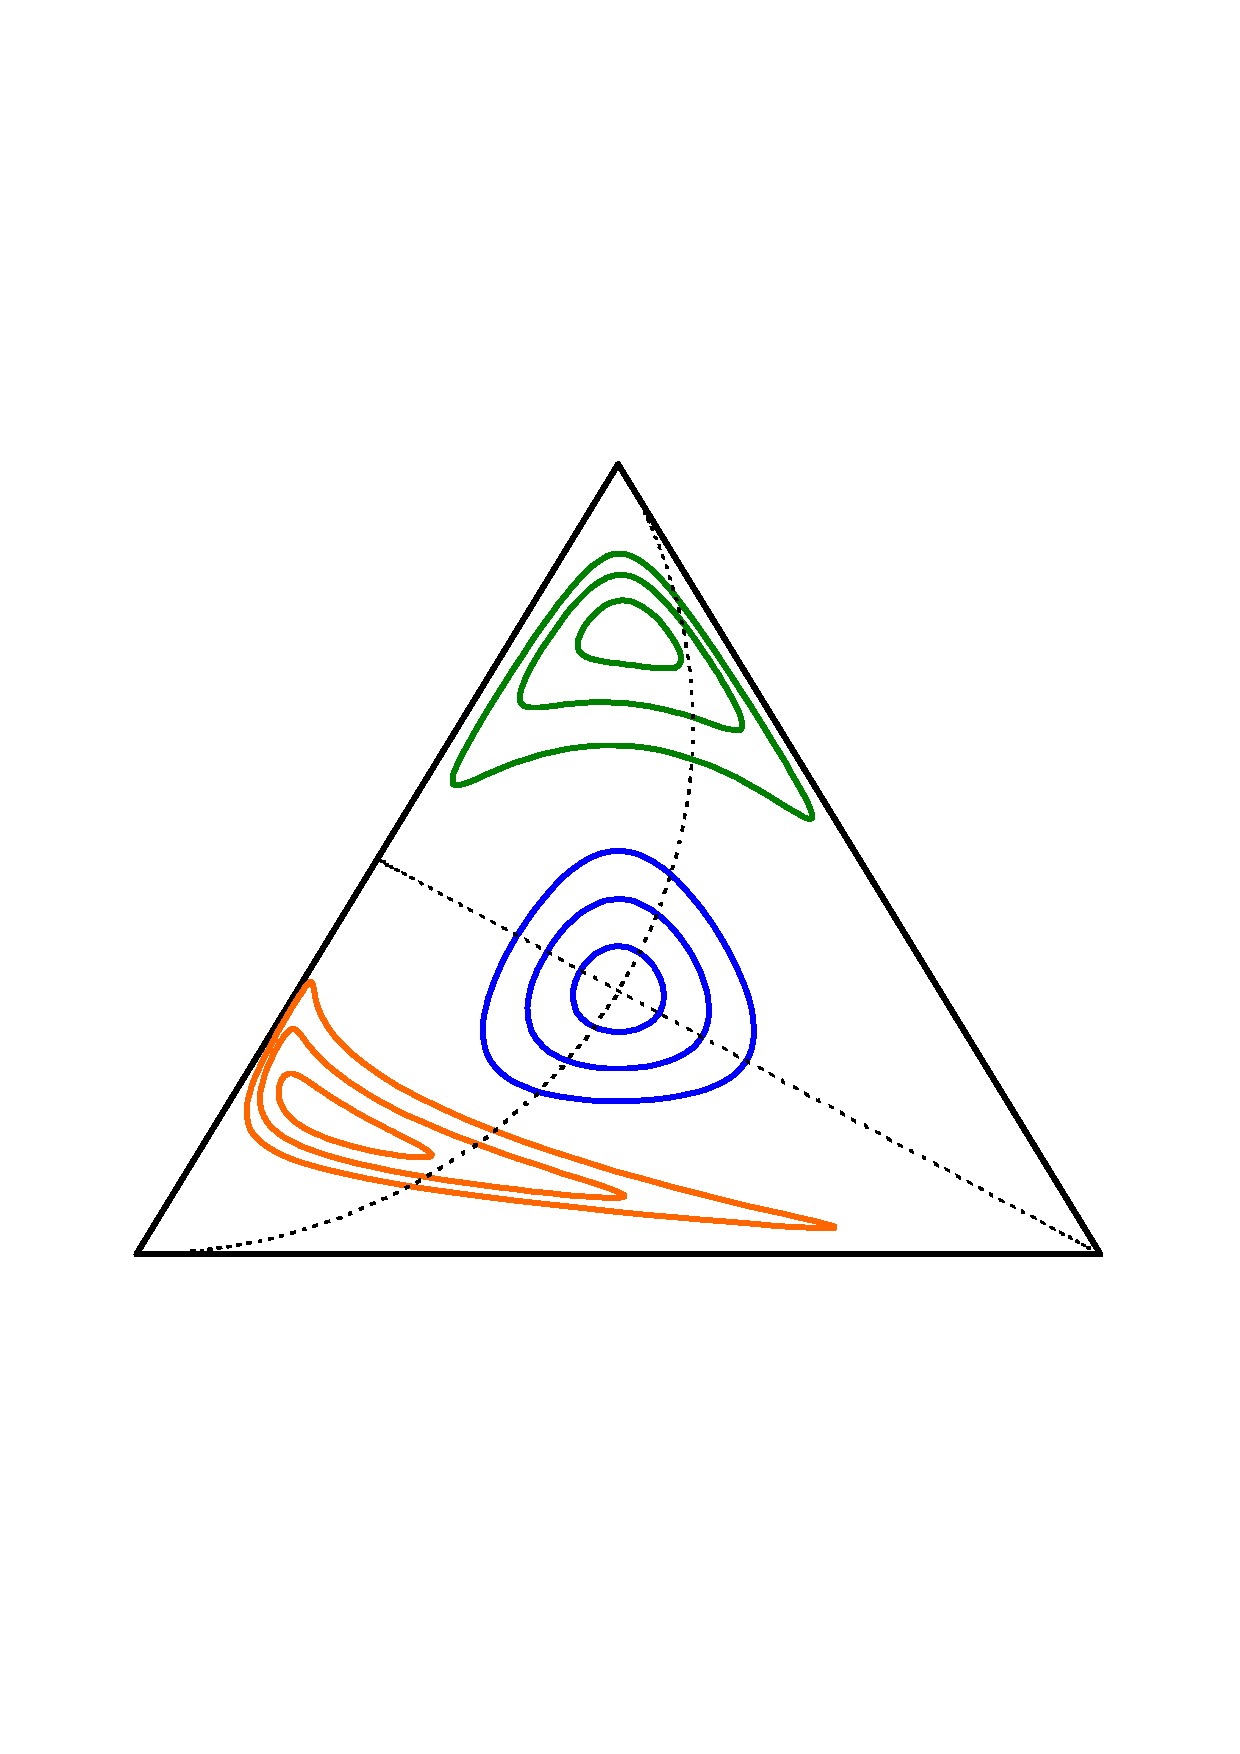
\includegraphics[trim=0cm 6cm 0cm 4cm,width=0.4\textwidth]{fig01_elipsesS3Axes.pdf} &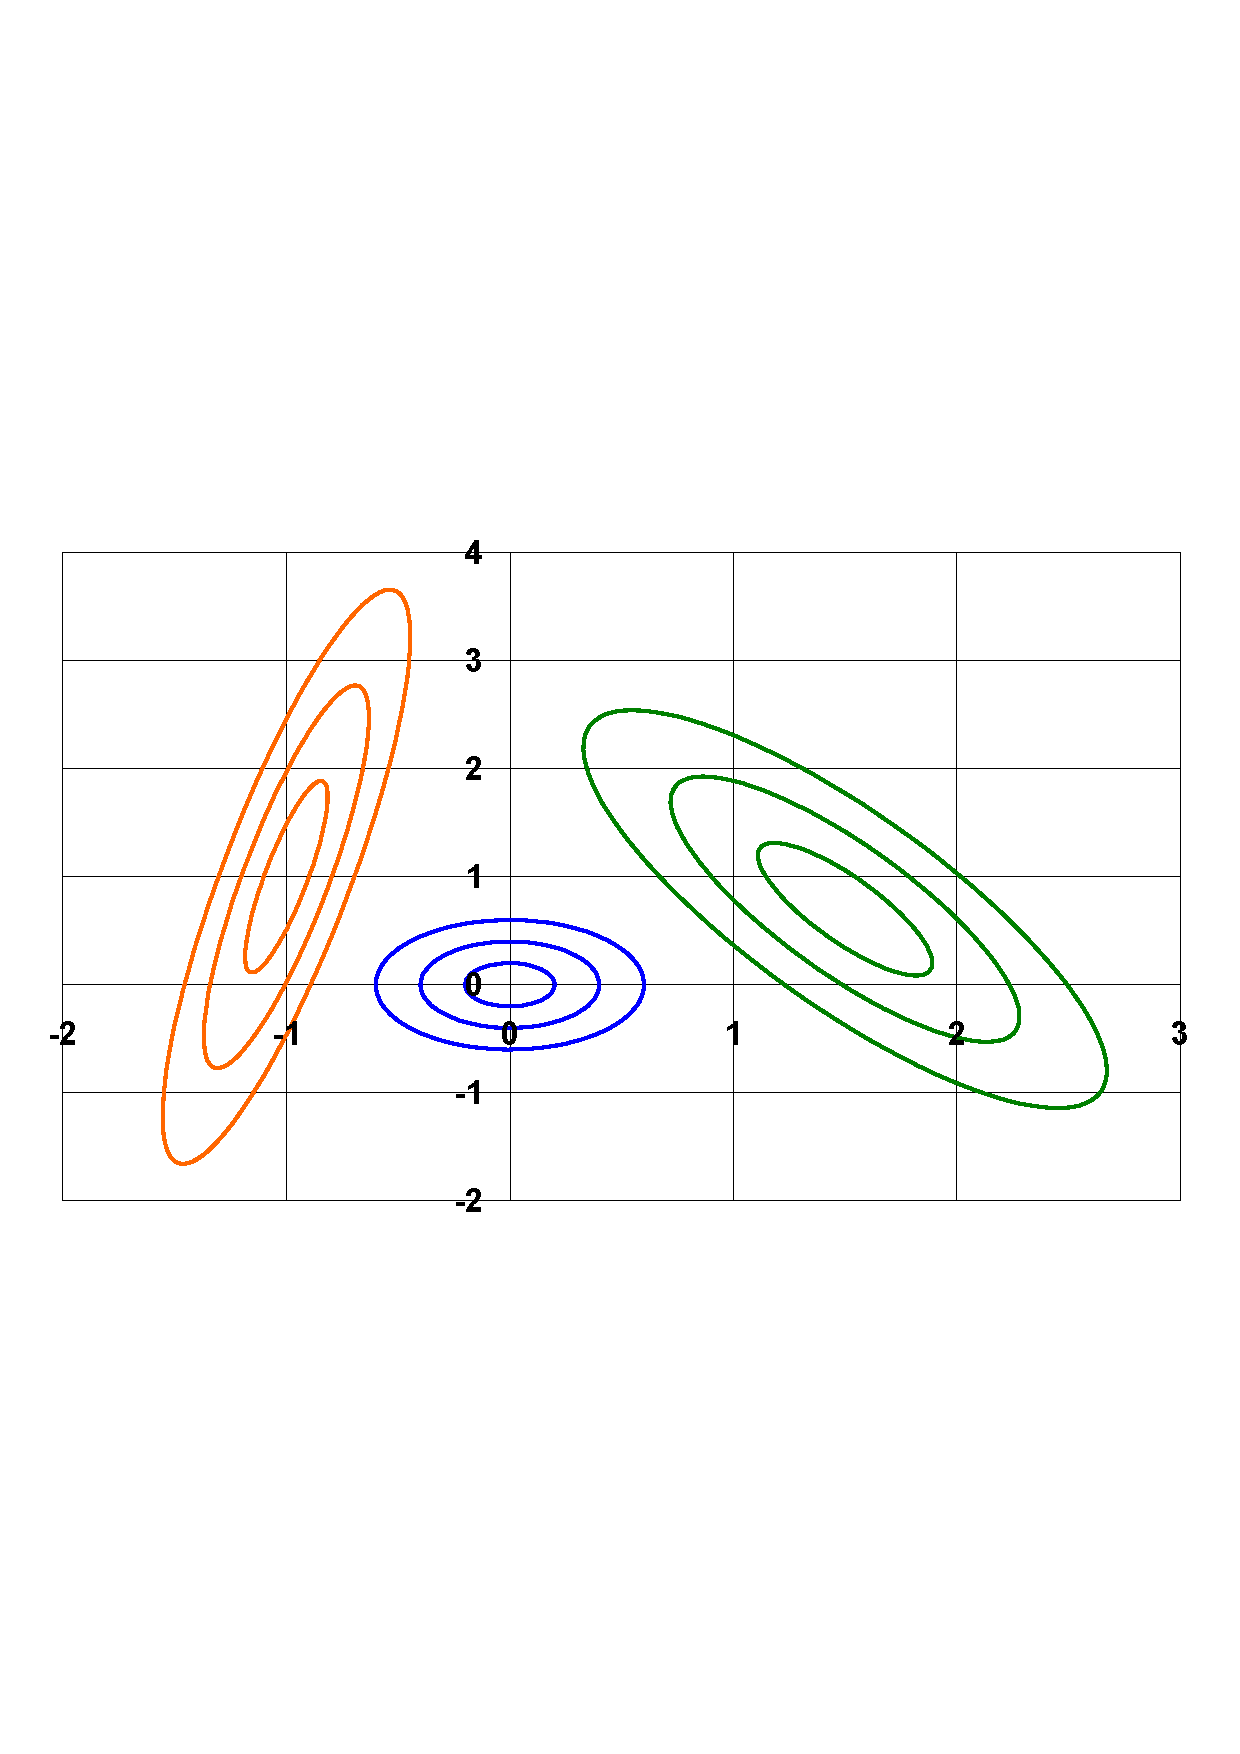
\includegraphics[trim=0cm 6cm 0cm 4cm,width=0.4\textwidth]{fig01_elipsesS3AxesC.pdf} \\
 \end{tabular}
 \caption{Contour lines of typical log-ratio normal distribution on the simplex: (left) in the ternary diagram. Dotted lines are the axis of log-ratio basis; (right) in coordinates. }\label{fig01}
\end{center}
\end{figure}


%\section{Mixtures on the simplex}

\section{Standard approaches to model composition data mixtures}
\label{standard_section}

\noindent Two different approaches have been used in the literature to fit finite mixtures to CoDa. 
In the first approach,  distributions defined on real space are used to define the mixture model and the special geometry of $\mathcal{S}^D$ is not considered. In the second approach,  the finite mixtures are based on Dirichlet distribution and its generalizations.


\subsection{Using distributions defined on the real space}
\label{real_section}

This approach consists in modelling CoDa using a mixture of distributions defined on the real space. Consequently the approach assumes that $\mathcal{S}^D$ is a subset of $\mathbb{R}^D$ and its particular Euclidean space structure described in Section 2 is not considered. Instead, the CoDa sample is assumed to be generated from a distribution with probability density given by Equation~\ref{mixt} where $f(\;\cdot\;;\theta_i): \mathbb{R}^D \rightarrow \mathbb{R}^+$ is a density function defined on the real space (a multivariate normal distributions, a  t-student distributions, etc).

The main advantage of using this approach is the simplicity of working without considering the restriction that every component must be positive.
Although this methodology has been applied in CoDa \citep[see][]{papageorgiou2001model}, it exhibits some limitations.


When CoDa is modelled using a mixture of distributions defined on the real space, neither the constant sum constraint nor the strictly positive component restriction is taken into an account. In fact, if we model a compositional sample using a mixture of densities defined on the real space, the mixture density is strictly positive in all the real space, and therefore, it is giving positive probability to impossible events. For example, it is straightforward to see that the \emph{impossible} event  of having the $i$-th component negative has positive probability, i.e $P(\{ \textbf{x} \in \mathcal{S}^d | x_i < 0 \}) > 0$. This difficulty is similar to the traditional confidence intervals of very small or very large proportions, they may provide values beyond the restricted space. 


Another limitation to deal with is the collinearity that appears between components  after restricting the components to sum a constant, see Eq. \ref{sum_to_constant}. The collinearity implies that the covariance matrix calculated from the sample is singular, and therefore, any method requiring that the covariance matrix is non singular can not be applied directly. Most mixture models are estimated using the EM-algorithm (citar McLachlan o Dempster). In the E-step, the algorithm needs to evaluate a density function computed from the sample. Because most densities depend on the inverse of the covariance matrix (multivariate normal, multivariate skew, etc), EM algorithm can not be applied directly. To solve this difficulty, a common approach consists on removing one part from the composition for the rest of the analysis \citep{papageorgiou2001model}. However, when one part is removed,  misleading result can be obtained. Suppose the following simple example: 

\begin{quote}
\begin{table}
\centering
\scriptsize
\input{tex/example-coda3.tex}
\label{example_elim_tab}
\caption{Dataset}
\end{table}

Consider a compositional sample $X$ with three components, $a$, $b$ and $c$ and $20$ observations (see Table~\ref{example_elim_tab}). Suppose that each observation comes from two possible sites, $S_1$ and $S_2$. Moreover, suppose that each observation is collected in two possible conditions, $C_1$ and $C_2$: in condition $C_1$ the level of element $c$ is lower than the level of element $c$ in condition $C_2$ (for example, consider element $c$ is water and condition $C_1$ is a sunny day while condition $C_2$ is a rainny day).

Sample $X$ is represented in Figure~\ref{example_elim_component}. In the ternary diagram it is not difficult to identify three groups: one formed with the observations collected in site $S_1$ (black and circular points), all of them collected under condition $C_1$, one with observations collected in site $S_2$ under condition $C_1$ (grey and circular) and another with observations collected in site $S_2$ under condition $C_2$ (grey and triangular).

\begin{figure}[thbp]
\centering
\includegraphics[trim=0cm 0cm 0cm 0cm,width=0.7\textwidth]{figures/example_ternary.pdf}
\caption{}\label{example_elim_component}
\end{figure}

Suppose a researcher is interested in fitting a mixture model to the compositional sample $X$. Because each observation $i$ has a perfect collinearity between components, $a_i+b_i+c_i = 100$, the standard multivariate normal density can not be evaluated. Because of this, the researcher decides to eliminate on component for the rest of the analysis. He does the following reasoning: ``Because component $c$ contains the effect of condition $C_1$ and $C_2$, and I am really interested on the relation between $a$ and $b$, I am going to eliminate component $c$''. After eliminating component $c$, the researcher ends up with the sample represented in Figure~\ref{example_elim_2_components}.

\begin{figure}[thbp]
\centering
\includegraphics[trim=0cm 0cm 0cm 0cm,width=0.7\textwidth]{figures/example_2component.pdf}
\caption{}\label{example_elim_2_components}
\end{figure}

Note that although the researcher was interested in analysing the relation between $a$ and $b$, when component $c$ is eliminated the effect of condition $C_1$ and $C_2$  is still present in the dataset. In Section~\ref{codamix_section} we go back to the example presenting a methodology which is coherent with this type of decision taken during an analysis.

\end{quote}
%Above difficulties suggest using appropriate probability distributions in mixture models for CoDa, distributions that take into account the constrained sample space.

\subsection{Using standard distributions defined on the simplex space}
\label{simplex_section}

\noindent Among all the distributions defined on the simplex (distributions with density function $f(\;\cdot\;;\theta): \mathcal{S}^D\rightarrow \mathbb{R}^+$), the Dirichlet distribution is the most widely used and well known. 
A Dirichlet distributed random vector is the projection into the simplex of a random vector formed by independent and equally scaled gamma distributed components. 
Despite its simplicity and its good mathematical properties, by construction it has a very strong independence structure \citep{aitchison1986statistical}. 
In practice, such independence structure heavily restricts Dirichlet potential modelling application. Most of real CoDa sets have
not this structure \citep{aitchison1986statistical}. To solve this difficulty, many generalizations of the Dirichlet distribution with less
independence structure have been proposed: the Connor and Mosimann's distribution
\citep{Connor:1969}, the scaled Dirichlet distribution \citep{aitchison1986statistical},  and the Liouville distribution \citep{rayens1994dependence}.  More recently, \cite{ongaro2008new} present the Flexible Dirichlet distribution, but future
developments are required to discover its potential application. Finally \cite{monti2011shifted} introduce the Shifted-scaled Dirichlet distribution. This generalized distribution is defined adding the operations
perturbation and powering (Eq. \ref{pert_pow}) to the standard Dirichlet distribution. Unfortunately all these attempts
have limited success to fit the general dependence structure of compositional data \citep{mateu2013normal}.

A finite mixture of distributions defined on the simplex space is a probability distribution with probability density function given by Eq.~\ref{mixt} where $f(\;\cdot\;;\theta)$, $f(\;\cdot\;;\theta): \mathcal{S}^D \rightarrow \mathbb{R}^+$, is a density function defined on the simplex space (Dirichlet, Generalized Dirichlet, etc).


In practice, there is no straightforward method to fit a Dirichlet mixture to a CoDa set (neither any of its generalizations). Indeed, contrary to the Gaussian case or mixtures defined on the real space, it is difficult to find in the literature routines or functions to fit a Dirichlet mixture. However, in the literature different methods are found to estimate the parameters of a Dirichlet. As the Dirichlet distribution is an exponential family, the log-likelihood function is globally concave and a global optimum can be obtained. According to \cite{ng2011dirichlet}, the MLE via Newton-Raphson algorithm converges to the global optimum. \cite{narayanan1991algorithm} provides a Fortran subroutine where three different possibilities are available to estimate the initial parameter required.
We can also obtain MLE estimates via the EM gradient methods \citep{ng2011dirichlet} or we can use a generalized method of moments
\citep{hansen1982large}.  
To obtain an approximation to the MLE estimator of a Dirichlet mixture, it is possible to apply the classification EM-algorithm \citep[CEM algorithm,][]{celeux1992classification} using any of the described approaches to fit a Dirichlet model.



\section{Modeling compositional data using a mixture of distributions defined on the log-ratio coordinates}
\label{codamix_section}

\noindent Our proposal consists in modelling CoDa using a finite mixtures of log-ratio distributions, i.e. to model CoDa with a probability density function given by 
\begin{equation}
\pi_1 f_\mathcal{B}(\;\cdot\; ; \theta_1) + \dots + \pi_k f_\mathcal{B}(\;\cdot\; ; \theta_k)
\label{codamixt}
\end{equation}

where $f_\mathcal{B}$ are probability density functions of log-ratio distributions as defined in Section~\ref{coda_section}. The main advantage of using this approach is that the nature of compositional data is taken into an account.

As in Section~\ref{coda_section}, assume $f_\mathcal{B}(\textbf{x} ; \theta) = f^*(h_\mathcal{B}(\textbf{x}) ; \theta)$. Given a CoDa sample $X =  \{ \textbf{x}_1, \textbf{x}_2, \dots , \textbf{x}_n \}$, fitting to the sample $X$ by maximum likelihood the parameters $\pi_1, \dots, \pi_k$ and $\theta_1, \dots, \theta_k$ of a finite mixture distribution with pdf given by Equation~\ref{codamixt} is equivalent to fitting by maximum likelihood the same parameters to the mixture distribution with pdf given by
\begin{equation}
\pi_1 f^*(\;\cdot\; ; \theta_1) + \dots + \pi_k f^*(\;\cdot\; ; \theta_k)
\label{coordmixt}
\end{equation}
using sample $X' = \{ h_\mathcal{B}(x_1), \dots, h_\mathcal{B}(x_n) \}$. Indeed, the likelihood function evaluated for sample $X$ in the probability density function given by Equation~\ref{codamixt} is

\begin{equation}
\prod_{i=1}^n \sum_{j=1}^k \pi_j f_\mathcal{B}(\textbf{x}_i; \theta_j),
\end{equation}

and by definition, $f_\mathcal{B}(\textbf{x} ; \theta) = f^*(h_\mathcal{B}(\textbf{x}) ; \theta)$, is equal to 

\begin{equation}\label{likeli}
\prod_{i=1}^n \sum_{j=1}^k \pi_j f^*(h_\mathcal{B}(\textbf{x}_i); \theta_j).
\end{equation}

It turns out that Equation~\ref{likeli} is the likelihood function evaluated for sample $X'$ in the probability density function given by Equation~\ref{coordmixt}. Because the likelihood functions are the same, likelihood estimators $\hat{\pi}_1, \dots, \hat{\pi}_k, \hat{\theta}_1, \dots, \hat{\theta}_k$ are also the same

\begin{eqnarray}
\hat{\pi}_1, \dots, \hat{\pi}_k, \hat{\theta}_1, \dots, \hat{\theta}_k = \argmax_{\pi_1, \dots, \pi_k, \theta_1, \dots, \theta_k} \prod_{i=1}^n \sum_{j=1}^k \pi_j f_\mathcal{B}(\textbf{x}_i; \theta_j) = \\ 
= \argmax_{\pi_1, \dots, \pi_k, \theta_1, \dots, \theta_k} \prod_{i=1}^n \sum_{j=1}^k \pi_j f^*(h_\mathcal{B}(\textbf{x}_i); \theta_j).
\end{eqnarray}

% When compositional data is modeled with mixtures of distributions defined on the log-ratio coordinates all the variables present in the analysis are taken into an account, and their relative
% 
% of working with coordinates is coherent

\begin{quote}

Going back to the example from Section~\ref{real_section}, we were interested in fitting a mixture to sample $X$ formed by components $a$, $b$ and $c$ (see Table~\ref{example_elim_tab}). We saw that to fit a mixture of distributions defined on the real space we had to eliminate one component. Moreover, we saw that the reason that motivated us to eliminate component $c$ was not fulfilled after eliminating the component.

Suppose a researcher is interested in fitting a mixture model  as explained in this section to the compositional sample $X$. Before starting his analysis, the researcher decides to work with the basis $\mathcal{B}$ of the simplex $\mathcal{S}^3$ defined, as in Section~\ref{coda_section}, as follows
\begin{equation}
\mathcal{B} = \left\{ \frac{1}{s_1}\Big( e^{1/\sqrt{2}}, 1/e^{\sqrt{1/2}}, 1 \Big), \; \frac{1}{s_2}\Big( e^{1/\sqrt{6}}, e^{1/\sqrt{6}}, 1/e^{\sqrt{2/3}} \Big) \right\},
\end{equation}
where $s_1 = e^{1/\sqrt{2}} + 1/e^{\sqrt{ 1/2}} + 1$ and $s_2= e^{1/\sqrt{6}} + e^{1/\sqrt{6}} + 1/e^{\sqrt{2/3}}$. 

With respect basis $\mathcal{B}$, the researcher expresses sample $X$ in coordinates 
\[X' = \{h_{\mathcal{B}}(\textbf{x}_1), \dots, h_{\mathcal{B}}(\textbf{x}_n)\}.\] In Table~\ref{example_ilr_tab} columns $h_1$ and $h_2$ contain the first and second coordinate of sample $X$ with respect basis $\mathcal{B}$ (i.e. $h_1 = \sqrt{1/2} \log(a/b)$ and $h_2 = \sqrt{2/3} \log(\sqrt{ab} / c)$), in Figure~\ref{example_ilr3} their representation. In the representation it is easy to identify the effect of each component.

\begin{table}
\centering
\scriptsize
\input{tex/example-coda3-ilr3.tex}
\caption{Dataset}
\label{example_ilr_tab}
\end{table}

\begin{figure}[thbp]
\centering
\includegraphics[trim=0cm 0cm 0cm 0cm,width=0.7\textwidth]{figures/example_ilr3.pdf}
\caption{}\label{example_ilr3}
\end{figure}

Suppose no that the researcher decides to eliminate component $c$ because he is not interested in which condition the sample was collected. After eliminating component $c$, he set a basis $\mathcal{B}'$ of $\mathcal{S}^2$ defined as in before
\begin{equation}
\mathcal{B}' = \left\{ \frac{1}{s_1}\Big( e^{1/\sqrt{2}}, 1/e^{\sqrt{1/2}} \Big) \right\},
\end{equation}
where $s_1 = e^{1/\sqrt{2}} + 1/e^{\sqrt{ 1/2}}$ and expresses component $a$ and $b$ in coordinates with respect the new basis. Doing so the researcher ends up with coordinates $h_1$ from Table~\ref{example_elim_tab} (note that the coordinates are the same as before). In Figure~\ref{example_ilr2} coordinate $h_1$ is represented. In the Figure it is easy to identify that all the sample collected on Site 1 are more or less in the same rank (between -1 and 0), by contrast the samples collected in Site 2 are close to one.

\begin{figure}[thbp]
\centering
\includegraphics[trim=0cm 0cm 0cm 0cm,width=0.7\textwidth]{figures/example_ilr2.pdf}
\caption{}\label{example_ilr2}
\end{figure}
% 
% %\textbf{v}_i = \frac{1}{s_i}\Big( \underbrace{e^{1/\sqrt{i(i+1)}}, \dots, e^{1/\sqrt{i(i+1)}}}_{i}, 1/e^{\sqrt{ i/(i+1)}}, \underbrace{1, \dots, 1}_{D-(i+1)} \Big) 
% \end{equation}
% %where $s_i =  i\,e^{1/\sqrt{i(i+1)}} + 1/e^{\sqrt{ i/(i+1)}} + D - (i+1)$

\end{quote}


%According to \cite{mateu2013normal}, in Equation \ref{likeliR} we are not applying a transformation $h$ to a composition, we only change its representation. 
%In consequence, the number of possible densities $f^*$ is  the same than in real space. 
%Due to its theoretical and computational simplicity, our first proposal is to use the normal distribution, i.e. we fit a Gaussian mixture to a CoDa set using as $f^*$ the log-ratio normal densities on $\mathcal{S}^D$  (Eq. \ref{eq:densSNormal}). However, in cases where asymmetric distributions provides a better fit, it is possible to use log-ratio skew-normal or log-ratio skew-t on $\mathcal{S}^D$. 

% Figure \ref{fig03logratiodens} shows a typical scenario where the purpose is to find groups in a data set. In this case there are for groups .......DESCRIURE LA SIMULACIO....
% 
% \begin{figure}[htbp]
% \centering
% 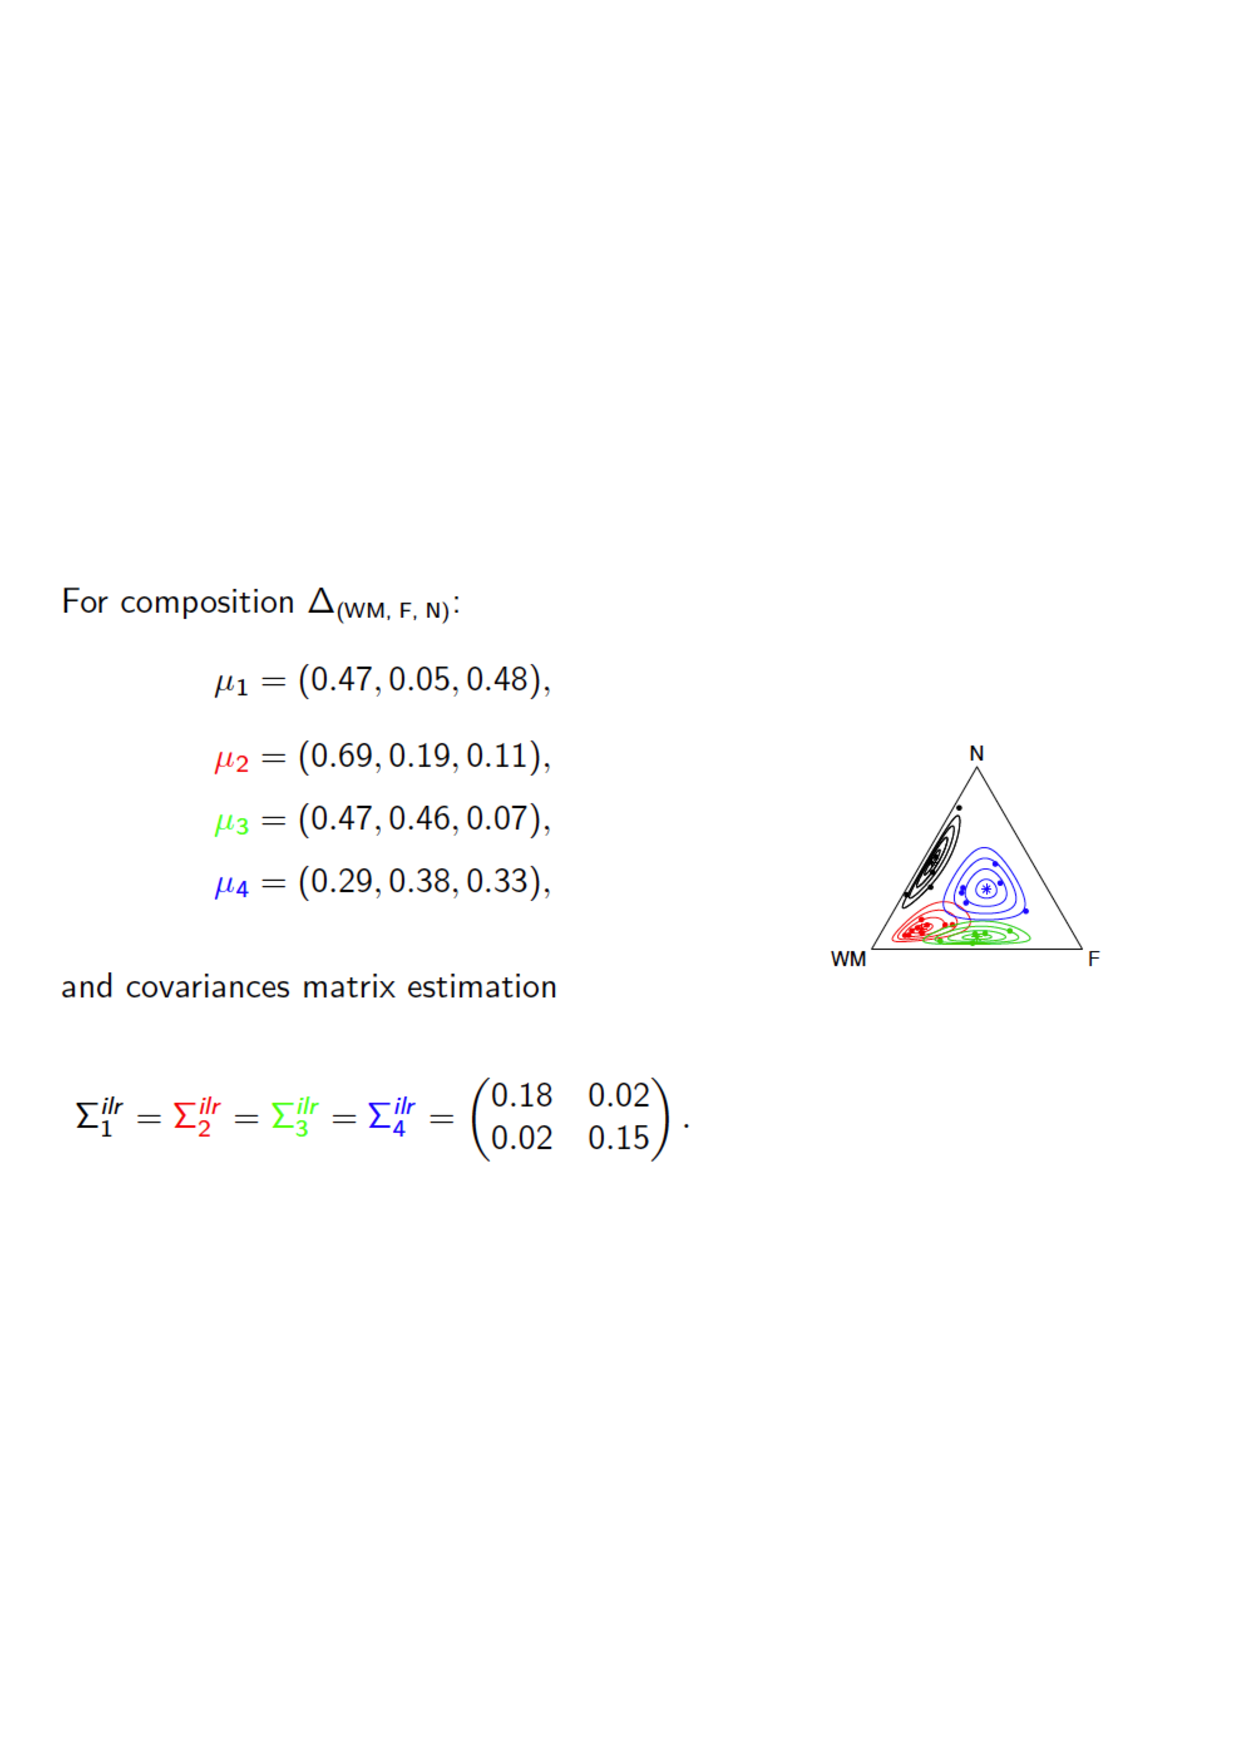
\includegraphics[trim=0cm 6cm 0cm 6cm,width=0.7\textwidth]{fig03_logratiodens.pdf}
% \caption{Typical model based clustering scenario using log-ratio normal distribution.}
% \label{fig03logratiodens}
% \end{figure}

It is important to remark that our method in most cases is basis invariant. That is, the fitted mixture are preserved when a change of basis and consequently a change of log-ratio coordinates is applied. For example, the log-ratio normal (Eq.~\ref{eq:densSNormal}) mixture model is formulated in terms of Mahalanobis distance and covariance matrix determinant which are basis invariant elements
 \citep{barcelo1999comment}.

 

\section{A real data set: Forensic Glass}
\label{example_section}

\noindent To illustrate and compare different approaches, we analyse the USA Forensic Science Service data set, also known as Forensic Glass data set. This data is available in UCI Machine Learning Repository \cite{Bache+Lichman:2013}.  The data set is composed by  $214$ glass samples where the percentages of eight chemical elements are provided. In addition, we have information about a grouping variable with seven levels, which splits the glass samples in seven groups. For our purposes, we only consider three chemical elements: Calcium (Ca), Silica (Si) and Aluminium (Al); and three groups of glasses: containers, headlamps and vehicle windows. We call this dataset Reduced Forensic Glass data set (\texttt{rfg}). Figure \ref{fig04} shows this data set formed by $59$ glass samples in the ternary diagram. Because the aluminium element takes small values the data set is close to the edge, inside the rectangle. For better illustration, Figure \ref{fig04} includes a zoom of the data set.


\begin{table}
\centering
\scriptsize
\input{tex/example-glasses-A.tex}
\quad
\input{tex/example-glasses-B.tex}
\label{example_elim_tab}
\caption{Dataset}
\end{table}


\begin{figure}[htbp]
\centering
\includegraphics[width=0.95\textwidth]{figures/main_df.pdf}%{fig04_original_solution2.pdf}
\caption{Forensic Glass data set in ternary diagram: Calcium (Ca), Silica (Si) and Aluminium (Al) chemical elements. Three groups of glasses: containers (black), headlamps (red) and vehicle windows (green).}
\label{fig04}
\end{figure}

For each different strategy a mixture of distributions with three components is adjusted to the given dataset.

\subsection*{Example: using distributions defined on the real space}

When dealing with real data, the most common mixture of distributions is the one with gaussian components. As commented in Section~\ref{real_section}, because of the collinearity inherent to CoDa ($\text{Ca}+\text{Si}+\text{Al} = 100$), to fit a gaussian mixture it is a common practice to eliminate one component. To fit a Gaussian mixture to \texttt{rfg} data set we eliminate the Calcium (Ca) component. After eliminating Ca component, we can fit a gaussian mixture using any standard package\footnote{for this example \texttt{Rmixmod} package has been used}, obtaining the gaussian mixture model with density function

\[
\pi_1 f(\;\cdot\; ; \mu_1, \Sigma_1) + \pi_2 f(\;\cdot\; ; \mu_2, \Sigma_2) + \pi_3 f(\;\cdot\; ; \mu_3, \Sigma_3)
\]

with parameters

{\small \input{tex/pars1_component_elimination.tex} }


Figure~\ref{fig05component_elimination} (top-left) shows the isodensity curves for the fitted mixture of gaussian distributions. The dashed line represents the limit of the simplex, i.e. the region were restrictions given by Equation~\ref{sum_to_constant} are held. In Figure~\ref{fig05component_elimination} (bottom-right) the isodensity curves have been completed to be represented in a ternary diagram. I the plot, it is clear that the distribution is giving positive probability to impossible regions. In Figure~\ref{fig05component_elimination} (top-right and bottom-left) are represented the isodensity curves resulting after removing Aluminium (Al) and Silica (Si) components respectively instead of Ca.

\begin{figure}[htbp]
\includegraphics[width=0.8\textwidth]{figures/elim_component_all.pdf}
\caption{USA Forensic Science Service data set considering only the subcomposition given by the Calcium (Ca), Silica (Si) and Aluminium (Al). On the top-left, top-right and bottom-left isodensity curves for mixtures of gaussian distributions in $R^{2}$ after removing the first, the second and the third component respectively. On bottom-right the isodensity curves transformed into the simplex.}
\label{fig05component_elimination}
\end{figure}

Despite the theoretical invariance of the maximum of the likelihood function wherever component we eliminate, we stated that in practice the numerical algorithm gets stuck in a local optimum. In such scenario, the invariance of the results is not guaranteed, and different mixture of Gaussian distributions can be obtained depending on the component we eliminate. 



\subsection*{Example: using standard distributions defined on the simplex space}

The Dirichlet distribution it is well kwown as a distribution defined on the simplex. To set a Dirichlet distribution in $\mathcal{S}^D$ it is necessary to specify its parameters $\left( \alpha^1 \dots \alpha^D \right)$. Therefore, to fit a mixture of $K$ Dirichlet distributions it is necessary to estimate the parameters $\pi_1$, \dots, $\pi_K$ and $\left( \alpha^1_1 \dots \alpha^D_1 \right), \dots, \left( \alpha^1_K \dots \alpha^D_K \right)$.

Fitting the parameters of a Dirichlet mixture it is not as easy as for the gaussian case. To ilustrate how the mixture of Dirichlet distributions fits to \texttt{rfg} dataset, we have approximate the MLE estimator of a Dirichlet mixture using the classification EM-algorithm proposed by \cite{celeux1992classification}. The obtained mixture of dirichlet distributions is given by

\[
\pi_1 f(\;\cdot\; ; \alpha_1) + \pi_2 f(\;\cdot\; \alpha_2) + \pi_3 f(\;\cdot\; ; \alpha_3)
\]

with parameters

{\small \input{tex/pars_dirichlet_mixture.tex} }


% \begin{small}
% \begin{tabbing}
% 0\=0123\=456\=789\=123456789012345\=67890123\=\kill
% \>\>\textbf{Classification EM algorithm to fit a Dirichlet mixture}\\
% \>\>\textbf{function} ($X$, $K$):\\
% \>\>\>Separate $X$ in $k$ disjoint sets $X_1, \dots, X_K$ at random\\
% \>\>\>\textbf{For} $i \in \{1,\dots,K\}$ \textbf{do}\\
% \>\>\>\>Fit parameters $\alpha^1_i, \dots, \alpha^K_i$ of a Dirichlet distribution to sample $X_i$\\
% \>\>\>\>Calculate $p_i$
% \end{tabbing}
% \end{small}


Figure~\ref{fig06fittingdirichlet} shows how a Dirichlet mixture fits the \texttt{rgf} dataset. Note that Dirichlet mixture is not be able to capture the dependence structure between the three chemical elements. 

\begin{figure}[htbp]
\centering
\includegraphics[width=0.95\textwidth]{figures/dirichlet_mixture.pdf}
\caption{USA Forensic Science Service data set: classification given by a standard Dirichlet mixture model. Three different groups of glasses: containers (black), headlamps (red) and vehicle windows (green)}
\label{fig06fittingdirichlet}
\end{figure}

\subsection*{Example: using distributions defined on the log-ratio coordinates}

Distributions defined on log-ratio coordinates allow to model data taking into account the nature of CoDa using standard distributions defined on real space.

To fit a mixture of distributions to \texttt{rfg} dataset it is necessary to express each composition respect a basis of $\mathcal{S}^3$. Let's consider basis 
\begin{equation}
\mathcal{B} = \left\{ \frac{1}{s_1}\Big( e^{1/\sqrt{2}}, 1/e^{\sqrt{1/2}}, 1 \Big), \; \frac{1}{s_2}\Big( e^{1/\sqrt{6}}, e^{1/\sqrt{6}}, 1/e^{\sqrt{2/3}} \Big) \right\},
\end{equation}
where $s_1 = e^{1/\sqrt{2}} + 1/e^{\sqrt{ 1/2}} + 1$ and $s_2= e^{1/\sqrt{6}} + e^{1/\sqrt{6}} + 1/e^{\sqrt{2/3}}$ as presented in Section~\ref{coda_section}. In Table~\ref{rgf_ilr}, \texttt{rgf} sample is expressed in coordinates respect basis $\mathcal{B}$, resulting in coordinates $h_1 = \sqrt{1/2} \log(\text{Ca}/\text{Si})$ and $h_2 = \sqrt{2/3} \log(\sqrt{\text{Ca} \cdot \text{Si}} / \text{Al})$. Respect coordinates $h_1$ and $h_2$ standard mixtures can be estimated.

\begin{table}
\centering
\scriptsize
\input{tex/example-glasses-ilr-A.tex}
\quad
\input{tex/example-glasses-ilr-B.tex}
\label{rgf_ilr}
\caption{Dataset}
\end{table}

Fitting a Gaussian mixture to the coordinates results in mixture model

\begin{equation}\label{coda_mixture}
\pi_1 f_{\mathcal{B}}(\cdot\;; \mu_1, \Sigma_1) + \pi_2 f_{\mathcal{B}}(\cdot\;; \mu_2, \Sigma_2) + \pi_3 f_{\mathcal{B}}(\cdot\;; \mu_3, \Sigma_3)
\end{equation}
with parameters

{\small \input{tex/pars_coda_gaussian_mixture.tex} }

Note that, although mixture model~\ref{coda_mixture} is defined on the Simplex, its parameters are defined respect coordinates $h_1$ and $h_2$. In Figure~\ref{fig07fittingcodaGaussian} the isocurves of density~\ref{coda_mixture} are represented.

\begin{figure}[htbp]
\centering
\includegraphics[width=\textwidth]{figures/coda_gaussian_mixture.pdf}\\
\caption{Compositional mixtures for USA Forensic Science Service data set: (top-left) Gaussian; (top-right) the same Gaussian mixture represented in the ternary; (bottom-left) skew-$t$ mixture; (bottom-right) the same skew-$t$ mixture represented in the ternary. }
\label{fig07fittingcodaGaussian}
\end{figure}



Following the same approach, it is not difficult to fit other models with different distributions than gaussian. In Figure~\ref{othercodadist} the mixture of other real defined distributions are represented with its representation in the Simplex.

\begin{figure}[htbp]
\centering
\includegraphics[width=0.8\textwidth]{figures/coda_skew_mixture.pdf}\\%{fig07_coda_skew_mixture2.pdf}
\includegraphics[width=0.8\textwidth]{figures/coda_skew_t_mixture.pdf}%{fig07_coda_skew_mixture2.pdf}
\caption{Compositional mixtures for USA Forensic Science Service data set: (top-left) Gaussian; (top-right) the same Gaussian mixture represented in the ternary; (bottom-left) skew-$t$ mixture; (bottom-right) the same skew-$t$ mixture represented in the ternary. }
\label{othercodadist}
\end{figure}


% To compare results, we fit normal and skew-t mixtures to the Forensic Glass data set. Figure~\ref{fig07fittingcodaGaussian} (top and bottom left) shows the isodensity contour plot of the fitted mixture in the space of log-ratio coordinates. Figure~\ref{fig07fittingcodaGaussian} (top and bottom right) shows the same contour lines in the ternary diagram.  It is important to note that we use the basis $\mathcal{B} = \{ (e^{-\sqrt{2}/2}, e^{\sqrt{2}/2}, e^{0}), (e^{-\sqrt{6}/6}, e^{-\sqrt{6}/6}, e^{\sqrt{6}/3}) \}$ on the simplex $\mathcal{S}^3$ and consequently the log-ratio coordinates in Eq. (\ref{eilr}). CAL DONAR RESULTATS??? Contrary to the Dirichlet case, both log-ratio mixtures are capable to capture the dependence structure of the data set. PERQU\`{E}?? CAL CONV\`{E}NCER MILLOR.
% 
% 
% \begin{figure}[htbp]
% \centering
% \includegraphics[width=0.6\textwidth]{figures/coda_gaussian_mixture.pdf}\\%{fig07_coda_gaussian_mixture2.pdf}\\
% %\caption{On the left Gaussian mixture fitted to the coordinates given the basis $\mathcal{B} = \{ (e^{-\sqrt{2}/2}, e^{\sqrt{2}/2}, e^{0}), (e^{-\sqrt{6}/6}, e^{-\sqrt{6}/6}, e^{\sqrt{6}/3}) \}$ of the simplex. On the right the same Gaussian mixture represented on the simplex.  }
% \includegraphics[width=0.6\textwidth]{figures/coda_skew_mixture.pdf}\\%{fig07_coda_skew_mixture2.pdf}
% \includegraphics[width=0.6\textwidth]{figures/coda_skew_t_mixture.pdf}%{fig07_coda_skew_mixture2.pdf}
% \caption{Compositional mixtures for USA Forensic Science Service data set: (top-left) Gaussian; (top-right) the same Gaussian mixture represented in the ternary; (bottom-left) skew-$t$ mixture; (bottom-right) the same skew-$t$ mixture represented in the ternary. }
% \label{fig07fittingcodaGaussian}
% \end{figure}


\section{Conclusions}
\label{conclusion_section}
Standard distributions in finite mixtures for compositional data sets show important difficulties. If densities for real data are used, probabilities to impossible events are obtained and the results depend on the removed part. Dirichlet density and some generalizations on the simplex can not capture the variability of many compositional data sets due to its strong independence structure. Log-ratio distributions are flexible models that could describe different form of variability and dependence structures. Indeed, any mixture model defined on the real space can be used to model data on the simplex space using the principle of working on coordinates. In particular, we have introduced the methodology to fit a mixture of normal and skew-$t$ distributions to the log-ratio coordinates of a compositional sample. This two options extend the range of possibilities we have up to now with the Dirichlet model or generalizations. The log-ratio normal distribution provides a rich enough parametric class of distributions on the appropriate sample space. 

\section*{Acknowledgments}
This research was supported by the Ministerio de Econom\'ia y Competividad under the project
``METRICS'' Ref. MTM2012-33236 and the Agència de Gestió d'Ajuts Universitaris i de Recerca (AGAUR), Generalitat de Catalunya (Ref: 2014SGR551).

%\section*{References}

\begin{thebibliography}{00}

\bibitem[Aitchison, 1986]{aitchison1986statistical}
Aitchison, J., 1986. The Statistical Analysis of Compositional Data. Monographs on Statistics and
Applied Probability. Chapman and Hall Ltd. (Reprinted 2003 with additional material by The
Blackburn Press), London (UK). 416 p.

\bibitem[Albert and Gupta, 1982]{albert1982mixtures}
Albert, J.~H. and Gupta, A.~K. (1982).
\newblock Mixtures of dirichlet distributions and estimation in contingency
  tables.
\newblock {\em The Annals of Statistics}, pages 1261--1268.

\bibitem[Andrews and McNicholas, 2012]{andrews2012model}
Andrews, J.~L. and McNicholas, P.~D. (2012).
\newblock Model-based clustering, classification, and discriminant analysis via
  mixtures of multivariate t-distributions.
\newblock {\em Statistics and Computing}, 22(5):1021--1029.

\bibitem[Bache and Lichman, 2013]{Bache+Lichman:2013}
Bache, K. and Lichman, M. (2013).
\newblock {UCI} machine learning repository.

\bibitem[Banerjee et~al., 2005]{banerjee2005clustering}
Banerjee, A., Dhillon, I.~S., Ghosh, J., and Sra, S. (2005).
\newblock Clustering on the unit hypersphere using von mises-fisher
  distributions.
\newblock In {\em Journal of Machine Learning Research}, pages 1345--1382.

\bibitem[Banfield and Raftery, 1993]{banfield1993model}
Banfield, J.~D. and Raftery, A.~E. (1993).
\newblock Model-based Gaussian and non-Gaussian clustering.
\newblock {\em Biometrics}, pages 803--821.

\bibitem[Barcel{\'o}-Vidal et~al., 1999]{barcelo1999comment}
Barcel{\'o}-Vidal, C., Mart{\'\i}n-Fern{\'a}ndez, J., and Pawlowsky-Glahn, V.
  (1999).
\newblock Comment on ``singularity and nonnormality in the classification of
  compositional data'' by gc bohling, jc davis, ra olea, and j. harff.
\newblock {\em Mathematical geology}, 31(5):581--585.

%\bibitem[Barcel{\'o}-Vidal et~al., 2011]{barcelo2011compositional}
%Barcelo-Vidal, C., Mart{\'\i}n-Fern{\'a}ndez, J.~A., and Mateu-Figueras, G.
%  (2011).
%\newblock Compositional differential calculus on the simplex.
%\newblock {\em Compositional Data Analysis: Theory and Applications, eds. V.
%  Pawlowsky-Glahn and A. Buccianti, John Wiley \& Sons, Ltd, Chichester, UK}.

\bibitem[Baudry et~al., 2010]{baudry2010combining}
Baudry, J.-P., Raftery, A.~E., Celeux, G., Lo, K., and Gottardo, R. (2010).
\newblock Combining mixture components for clustering.
\newblock {\em Journal of Computational and Graphical Statistics}, 19(2).

\bibitem[Bickel and Scheffer, 2004]{bickel2004multi}
Bickel, S. and Scheffer, T. (2004).
\newblock Multi-view clustering.
\newblock In {\em ICDM}, volume~4, pages 19--26.

%\bibitem[Bouguila, 2008]{bouguila2008clustering}
%Bouguila, N. (2008).
%\newblock Clustering of count data using generalized dirichlet multinomial
%  distributions.
%\newblock {\em Knowledge and Data Engineering, IEEE Transactions on},
%  20(4):462--474.

\bibitem[Bouguila, 2011]{bouguila2011count}
Bouguila, N. (2011).
\newblock Count data modeling and classification using finite mixtures of
  distributions.
\newblock {\em Neural Networks, IEEE Transactions on}, 22(2):186--198.

\bibitem[Bouguila et~al., 2004]{bouguila2004unsupervised}
Bouguila, N., Ziou, D., and Vaillancourt, J. (2004).
\newblock Unsupervised learning of a finite mixture model based on the
  dirichlet distribution and its application.
\newblock {\em Image Processing, IEEE Transactions on}, 13(11):1533--1543.

\bibitem[Bouveyron and Brunet-Saumard, 2014]{bouveyron2014model}
Bouveyron, C. and Brunet-Saumard, C. (2014).
\newblock Model-based clustering of high-dimensional data: a review.
\newblock {\em Computational Statistics and Data Analysis}, 71:52--78.

\bibitem[Browne and McNicholas, 2014]{browne2013mixture}
Browne, R. and McNicholas, P. (submitted).
\newblock A mixture of generalized hyperbolic distributions. arxiv: 13051036.

\bibitem[Buccianti, 2011]{Buccianti11}
Buccianti, A. (2011). 
\newblock Natural Laws Governing the Distribution of the Elements in Geochemistry: the Role of the Log-ratio Approach.
\newblock In {\em Compositional Data Analysis: Theory
and Applications}, eds. V. Pawlowsky-Glahn and A. Buccianti; Chichester, UK: John Wiley and Sons, 255--266.

\bibitem[Celeux and Govaert, 1992]{celeux1992classification}
Celeux, G. and Govaert, G. (1992).
\newblock A classification em algorithm for clustering and two stochastic
  versions.
\newblock {\em Computational statistics and Data analysis}, 14(3):315--332.

\bibitem[Comas-Cuf\'i et~al., 2013]{CMM13}
Comas-Cuf\'i, C., Mateu-Figueras, G., and Mart\'in-Fern\'andez, J. (2013).
\newblock Compositional entropies in model based clustering.
\newblock In {\em Abstracts of the 6th International Conference of the ERCIM WG
  on COMPUTING \& STATISTICS (ERCIM 2013)}. 14-16 December 2013, University of
  London, UK.

\bibitem[Connor and Mosimann, 1969]{Connor:1969}
Connor, R. and Mosimann, J. (1969).
\newblock Concepts of independence for proportions with a generalization of the
  {D}irichlet distribution.
\newblock {\em Journal of the American Statistical Association},
  64(325):194--206.

\bibitem[Egozcue et~al., 2003]{egozcue2003isometric}
Egozcue, J.~J., Pawlowsky-Glahn, V., Mateu-Figueras, G., and Barcel{\'o}-Vidal,
  C. (2003).
\newblock Isometric logratio transformations for compositional data analysis.
\newblock {\em Mathematical Geology}, 35(3):279--300.

\bibitem[Egozcue and Pawlowsky, 2005]{egozcue2005balances}
Egozcue, J.~J., and Pawlowsky-Glahn, V. (2005).
\newblock Groups of parts and their balances in compositional data analysis.
\newblock {\em Mathematical Geology}, 37(7):795--828.

\bibitem[Fraley and Raftery, 2002]{fraley2002model}
Fraley, C. and Raftery, A.~E. (2002).
\newblock Model-based clustering, discriminant analysis, and density
  estimation.
\newblock {\em Journal of the American Statistical Association},
  97(458):611--631.

\bibitem[Hansen, 1982]{hansen1982large}
Hansen, L.~P. (1982).
\newblock Large sample properties of generalized method of moments estimators.
\newblock {\em Econometrica: Journal of the Econometric Society}, pages
  1029--1054.

\bibitem[Lee and McLachlan, 2011]{lee2011fitting}
Lee, S. and McLachlan, G.~J. (2011).
\newblock On the fitting of mixtures of multivariate skew t-distributions via
  the em algorithm.
\newblock {\em arXiv preprint arXiv:1109.4706}.

\bibitem[Lee and McLachlan, 2013]{lee2013finite}
Lee, S. and McLachlan, G.~J. (2013).
\newblock Finite mixtures of multivariate skew t-distributions: some recent and
  new results.
\newblock {\em Statistics and Computing}, pages 1--22.

\bibitem[Lin, 2010]{lin2010robust}
Lin, T.-I. (2010).
\newblock Robust mixture modeling using multivariate skew t distributions.
\newblock {\em Statistics and Computing}, 20(3):343--356.

%\bibitem[Lin et~al., 2007]{lin2007robust}
%Lin, T.~I., Lee, J.~C., and Hsieh, W.~J. (2007).
%\newblock Robust mixture modeling using the skew t distribution.
%\newblock {\em Statistics and Computing}, 17(2):81--92.

\bibitem[Mardia et~al., 2007]{mardia2007protein}
Mardia, K.~V., Taylor, C.~C., and Subramaniam, G.~K. (2007).
\newblock Protein bioinformatics and mixtures of bivariate von mises
  distributions for angular data.
\newblock {\em Biometrics}, 63(2):505--512.

\bibitem[Mart\'in-Fern\'andez et~al., 2012]{M+12}
Mart\'in-Fern\'andez, J., Hron, K., Templ, M., Filzmoser, P., and
  Palarea-Albaladejo (2012).
\newblock Model-based replacement of rounded zeros in compositional data:
  Classical and robust approach.
\newblock {\em Computational Statistics \& Data Analysis}, 56(3):2688--2704.

\bibitem[Mateu-Figueras and Pawlowsky-Glahn, 2007]{mateu2007skew}
Mateu-Figueras, G. and Pawlowsky-Glahn, V. (2007).
\newblock The skew-normal distribution on the simplex.
\newblock {\em Communications in Statistics, Theory and Methods, Special Issue
  Skew-elliptical Distributions and Their Application}, 36(9):1787--1802.

\bibitem[Mateu-Figueras et~al., 2011]{MPE2011}
Mateu-Figueras, G., Pawlowsky-Glahn, V., and Egozcue, J. (2011).
\newblock The principle of working on coordinates.
\newblock In {\em Compositional Data Analysis: Theory and Applications}, pages
  31--42. John Wiley \& Sons.

\bibitem[Mateu-Figueras et~al., 2013]{mateu2013normal}
Mateu-Figueras, G., Pawlowsky-Glahn, V., and Egozcue, J.-J. (2013).
\newblock The normal distribution in some constrained sample spaces.
\newblock {\em SORT-Statistics and Operations Research Transactions},
  1(1):29--56.

\bibitem[McLachlan and Peel, 2004]{mclachlan2004finite}
McLachlan, G. and Peel, D. (2004).
\newblock {\em Finite mixture models}.
\newblock Wile.

%\bibitem[McLachlan and Basford, 1988]{mclachlan1988mixture}
%McLachlan, G.~J. and Basford, K.~E. (1988).
%\newblock Mixture models. inference and applications to clustering.
%\newblock {\em Statistics: Textbooks and Monographs, New York: Dekker, 1988},
%  1.

\bibitem[Monti et~al., 2011]{monti2011shifted}
Monti, G., Mateu-Figueras, G., Pawlowsky-Glahn, V., and Egozcue, J. (2011).
\newblock The shifted-scaled dirichlet distribution in the simplex.
\newblock In {\em Proceedings of the 4th International Workshop on
  Compositional Data Analysis (2011)}.

\bibitem[Narayanan, 1991]{narayanan1991algorithm}
Narayanan, A. (1991).
\newblock Algorithm as 266: maximum likelihood estimation of the parameters of
  the dirichlet distribution.
\newblock {\em Journal of the Royal Statistical Society. Series C (Applied
  Statistics)}, 40(2):365--374.

\bibitem[Ng et~al., 2011]{ng2011dirichlet}
Ng, K.~W., Tian, G.-L., and Tang, M.-L. (2011).
\newblock {\em Dirichlet and Related Distributions: Theory, Methods and
  Applications}, volume 888.
\newblock John Wiley \& Sons.

\bibitem[Ongaro et~al., 2008]{ongaro2008new}
Ongaro, A., Migliorati, S., Monti, G.~S., et~al. (2008).
\newblock A new distribution on the simplex containing the dirichlet family.
\newblock Technical report, Universitat de Girona. Departament
  d'Inform{\`a}tica i Matem{\`a}tica Aplicada.

\bibitem[Papageorgiou et~al., 2001]{papageorgiou2001model}
Papageorgiou, I., Baxter, M., and Cau, M. (2001).
\newblock Model-based cluster analysis of artefact compositional data.
\newblock {\em Archaeometry}, 43(4):571--588.

%\bibitem[Pavlov et~al., 2004]{pavlov2004document}
%Pavlov, D., Balasubramanyan, R., Dom, B., Kapur, S., and Parikh, J. (2004).
%\newblock Document preprocessing for naive bayes classification and clustering
%  with mixture of multinomials.
%\newblock In {\em Proceedings of the tenth ACM SIGKDD international conference
%  on Knowledge discovery and data mining}, pages 829--834. ACM.

\bibitem[Pawlowsky-Glahn and Egozcue, 2001]{PE01}
Pawlowsky-Glahn, V. and Egozcue, J. (2001).
\newblock Geometric approach to statistical analysis on the simplex.
\newblock {\em Stochastic Environmental Research and Risk Assessment (SERRA)},
  15(5):384--398.

\bibitem[R~Core~Team, 2013]{R2013soft}
R Core Team (2013).
\newblock R: A language and environment for statistical computing. R Foundation for Statistical Computing.
\newblock {\em Vienna, Austria. \texttt{http://www.R-project.org/}}.

\bibitem[Rayens and Srinivasan, 1994]{rayens1994dependence}
Rayens, W.~S. and Srinivasan, C. (1994).
\newblock Dependence properties of generalized liouville distributions on the
  simplex.
\newblock {\em Journal of the American Statistical Association},
  89(428):1465--1470.

\bibitem[Scott and Symons, 1971]{scott1971clustering}
Scott, A. and Symons, M.~J. (1971).
\newblock Clustering methods based on likelihood ratio criteria.
\newblock {\em Biometrics}, pages 387--397.

\bibitem[Tian et~al., 2003]{tian2003bayesian}
Tian, G.-L., Ng, K.~W., and Geng, Z. (2003).
\newblock Bayesian computation for contingency tables with incomplete
  cell-counts.
\newblock {\em Statistica Sinica}, 13(1):189--206.

\end{thebibliography}

\newpage
\appendix
\section{Basis invariance}

\begin{prop}
Let $\mathcal{B}$ be an orthonormal basis. Let  $\Theta$ be a parameter space. Let $f(\textbf{x} ; \theta_{\mathcal{B}})$ be a probability density function defined on the simplex space $\mathcal{S}^D$ with $\theta_{\mathcal{B}} \in \Theta$.

If for any orthogonal matrix $Q$ there is a parameter $\theta' \in \Theta$ such that 
\[
\forall \textbf{x} \in \mathcal{S}^D, \;\; f^*(h_\mathcal{B}(\textbf{x}) \cdot Q ;\; \theta') = f(\textbf{x};\; \theta) 
\]
then the probability function $f$ is basis invariant.
\end{prop}

\end{document}

\endinput 
